\documentclass[xcolor=dvipsnames,beamer]{beamer} %handout,notes=show

\usepackage{textcomp}
\usepackage[utf8]{inputenc}
% \usepackage{default}
\usepackage{graphicx}
%  \usepackage[pdftex]{hyperref}
\usepackage{url}
\usepackage{amsmath}

% frames have to be fragile
\newif\ifnotes
\input{tmpnotessettings}
%\notestrue


\ifnotes
%\setbeamertemplate{note page}[plain]
\setbeamertemplate{note page}[compress]
\setbeamerfont{note page}{size=\large}
\setbeameroption{show only notes}
%\setbeameroption{show notes}
\usepackage{pgfpages}
\pgfpagesuselayout{2 on 1}[a4paper,border shrink=5mm]%
\else
%\setbeameroption{hide notes}
\fi
%\notesfalse



% nastaveni TypeWriter
%\usepackage{courier}
%\usepackage{lmodern}
%\renewcommand*\ttdefault{txtt}
\DeclareFontShape{OT1}{cmtt}{bx}{n}{<5><6><7><8><9><10><10.95><12><14.4><17.28><20.74><24.88>cmttb10}{}


% \usepackage{verbatim}
\usepackage[absolute,overlay]{textpos}

\usepackage{listings}
% \usepackage{courier}
\definecolor{grey}{RGB}{70,70,70}
\definecolor{green}{RGB}{0,255,0}
\definecolor{red}{RGB}{202,53,53}
\definecolor{lightGrey}{RGB}{250,250,250}
\definecolor{darkGrey}{RGB}{50,50,50}


\usepackage{color}
\definecolor{lightgray}{rgb}{.9,.9,.9}
\definecolor{darkgray}{rgb}{.4,.4,.4}
\definecolor{purple}{rgb}{0.65, 0.12, 0.82}

% \usetheme{Boadilla}
\usetheme{Goettingen}
% \usetheme{Montpellier}
% \usetheme{Warsaw}
% \usetheme{Madrid}
% \usetheme{Szeged}
% \useoutertheme{infolines}
% \usecolortheme[named=MidnightBlue]{structure}
\usecolortheme[named=PineGreen]{structure}
% \setbeamertemplate{navigation symbols}{}




\title[Titan Meth. Cycle]
{\vspace{70pt}
(M)ethanological cycle of Titan}
%\subtitle{Mini-project ATPS}
%\pdforstring{}{}
\author[Yann Chemin]
{\vspace{40pt}\\
Mini-project ATPS}

\institute[BBK]
{B.Sc. Planetary Sciences with Astronomy \\
 \vspace{5pt}
 $3^{rd}$ Year,  Advanced Topics of Planetary Sciences
\begin{center}
 \includegraphics[width=2.5cm]{Birkbeck}
\end{center}
}
\date{\tiny \textcolor{white}{February 23rd, 2014}}


%\AtBeginSection[]{\begin{frame}\frametitle{Obsah}%
%\tableofcontents[currentsection ]\end{frame}}
%\AtBeginSubsection[]
%{
%  \begin{frame}<beamer>
%  \frametitle{Obsah}
%  \tableofcontents[currentsection,currentsubsection]
%  \end{frame}
%}

\setbeamercovered{transparent}

\hypersetup{%
	pdfauthor={Yann Chemin},%
	pdfsubject={Presentation},%
    pdfkeywords={Titan, methane, ethane, cycle, rainfall, evaporation, run-off, erosion, climate}
}

\input{nastavenilst}

\newcommand{\overovaciref}[1]{{\scriptsize(\ref{#1})}}


\usepackage{tipa}
\newcommand{\pron}[2]{#1 [#2]}

%%%%%%%%%%%%%%%%%%%%%%%%%%%%%%%%%%%%%%%%%%%%%%%%%%%%%%%%%%%%%%%%%%%%
% TOC frame setup
%%%%%%%%%%%%%%%%%%%%%%%%%%%%%%%%%%%%%%%%%%%%%%%%%%%%%%%%%%%%%%%%%%%%
\usepackage{multicol}
\colorlet{mycolor}{orange!80!black}% change this color to suit your needs
\AtBeginSection[]{
  \setbeamercolor{section in toc shaded}{use=structure,fg=structure.fg}
  \setbeamercolor{section in toc}{fg=mycolor}
  \setbeamercolor{subsection in toc shaded}{fg=black}
  \setbeamercolor{subsection in toc}{fg=mycolor}
  \frame<beamer>{\begin{multicols}{2}
  \frametitle{Outline}
  \setcounter{tocdepth}{2}  
  \tableofcontents[currentsection,subsections]
\end{multicols} 
 }
}

\setbeamercolor{author in head/foot}{fg=white}
\setbeamercolor{title in head/foot}{fg=white}
\setbeamercolor{section in head/foot}{fg=mycolor}
\setbeamertemplate{section in head/foot shaded}{\color{white!70!black}\insertsectionhead}
\setbeamercolor{subsection in head/foot}{fg=mycolor}
\setbeamertemplate{subsection in head/foot shaded}{\color{white!70!black}\insertsubsectionhead}
\setbeamercolor{frametitle}{fg=white}
\setbeamercolor{framesubtitle}{fg=white}

%%%%%%%%%%%%%%%%%%%%%%%%%%%%%%%%%%%%%%%%%%%%%%%%%%%%%%%%%%%%%%%%%%%%
%%%%%%%%%%%%%%%%%%%%%%%%%%%%%%%%%%%%%%%%%%%%%%%%%%%%%%%%%%%%%%%%%%%%
%%%%%%%%%%%%%%%%%%%%%%%%%%%%%%%%%%%%%%%%%%%%%%%%%%%%%%%%%%%%%%%%%%%%
\begin{document}


%%%%%%%%%%%%%%%%%%%%%%%%%%%%%%%%%%%%%%%%%%%%%%%%%%%%%%%%%%%%%%%%%%%%
\begin{frame}
 \maketitle
\end{frame}
%%%%%%%%%%%%%%%%%%%%%%%%%%%%%%%%%%%%%%%%%%%%%%%%%%%%%%%%%%%%%%%%%%%%

%%%%%%%%%%%%%%%%%%%%%%%%%%%%%%%%%%%%%%%%%%%%%%%%%%%%%%%%%%%%%%%%%%%%
\begin{frame}{Contents}
 \begin{multicols}{2}
  \setcounter{tocdepth}{2}  
  \tableofcontents
 \end{multicols} 
\end{frame}
%%%%%%%%%%%%%%%%%%%%%%%%%%%%%%%%%%%%%%%%%%%%%%%%%%%%%%%%%%%%%%%%%%%%

\section{Titan}
%%%%%%%%%%%%%%%%%%%%%%%%%%%%%%%%%%%%%%%%%%%%%%%%%%%%%%%%%%%%%%%%%%%%
\begin{frame}[fragile]{Titan}
\begin{block}{Titan (Saturn VI)}
 The largest of Saturn’s natural satellites\\
 1.5 times the diameter of the Moon
\end{block}
\begin{block}{Hydrocarbons}
 Surface and atmospheric hydrocarbon\\
 Methane ($CH_4$) of solar system origins\\
 Ethane ($C_2H_6$) rainfall
\end{block}
\begin{block}{Hydrocarbons}
 Triple phase temperature range (solid, liquid, gas)\\
 Atmospheric photolysis of $CH_4$ to $C_2H_6$\\
 Oceans \& Lakes as source of atmospheric content
\end{block}
\end{frame}


\section{Energy Balance}
\subsection{Atm. Layers}
%%%%%%%%%%%%%%%%%%%%%%%%%%%%%%%%%%%%%%%%%%%%%%%%%%%%%%%%%%%%%%%%%%%%
\begin{frame}[fragile]{Titan Atmospheric Layers}

\begin{center}
 \includegraphics[width=7.5cm]{images/Titan_Many_Layers}
\end{center}
\noindent {\tiny \it Image Credit: NASA/JPL-Caltech\\http://photojournal.jpl.nasa.gov/jpeg/PIA06160.jpg}
\end{frame}

\subsection{Atm. Profile}
%%%%%%%%%%%%%%%%%%%%%%%%%%%%%%%%%%%%%%%%%%%%%%%%%%%%%%%%%%%%%%%%%%%%
\begin{frame}[fragile]{Atmospheric Profile}

\begin{center}
  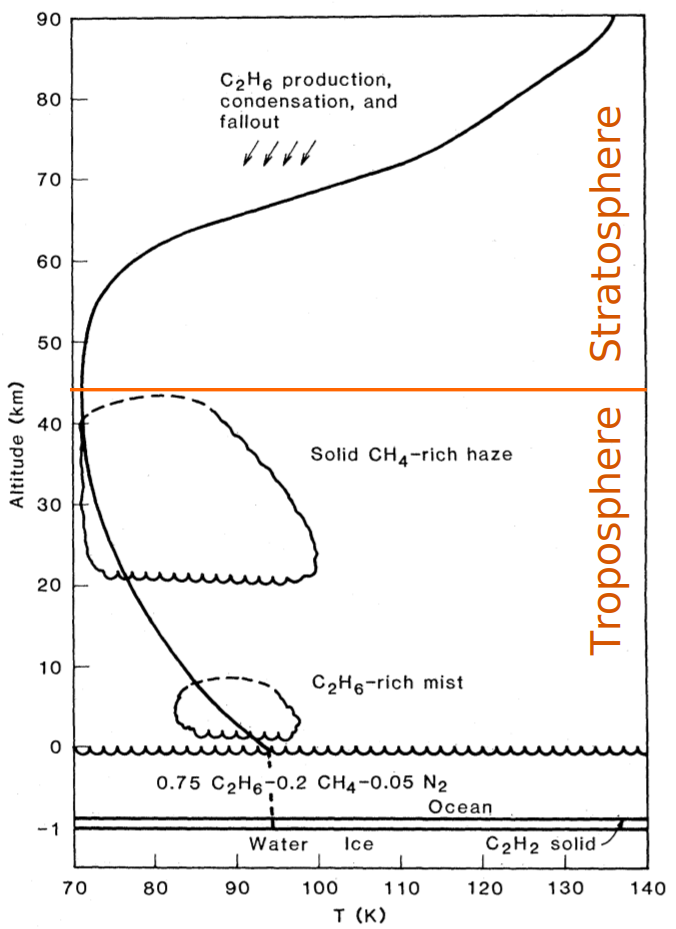
\includegraphics[width=5.5cm]{images/1983_Lunine_et_al}
\end{center}
\noindent {\tiny \it Figure Credit: Lunine et al. (1983)}
\end{frame}

\subsection{Radiation Budget}
%%%%%%%%%%%%%%%%%%%%%%%%%%%%%%%%%%%%%%%%%%%%%%%%%%%%%%%%%%%%%%%%%%%%
\begin{frame}[fragile]{Radiation Budget}
\begin{block}{The generic longwave greybody/blackbody radiation:}
\begin{equation}
 GE = \varepsilon BB = \varepsilon \sigma T^4
\end{equation}
\end{block}
\begin{block}{The radiation budget at planetary surface:}
\begin{equation}
 R_{net} = SW_{bal} + LW_{bal}
\end{equation}
\end{block}
\begin{block}{Radiation budget generic extension at planetary surface:}
\begin{equation}
 R_{net} =(1-\rho)\tau_{sw} E_s+(1-\varepsilon_0) \sigma T_{0}^4+(\varepsilon_{atm}-1) \sigma T_{atm}^4+\epsilon
\end{equation}
\end{block}
This provides the constraint on the available energy for conduction, convection and vaporization processes at surface
\end{frame}

\subsection{Energy Budget}
%%%%%%%%%%%%%%%%%%%%%%%%%%%%%%%%%%%%%%%%%%%%%%%%%%%%%%%%%%%%%%%%%%%%
\begin{frame}[fragile]{Energy Budget}

\begin{center}
 \includegraphics[width=7.3cm]{images/energybalance}
\end{center}
\noindent {\tiny \it Figure Credit: recreated after McKay et al. (1991)}
\end{frame}

\section{Oceans \& Lakes}
\subsection{Polar lakes}
%%%%%%%%%%%%%%%%%%%%%%%%%%%%%%%%%%%%%%%%%%%%%%%%%%%%%%%%%%%%%%%%%%%%
\begin{frame}[fragile]{North Pole}

\begin{center}
  \includegraphics[width=8.7cm]{images/TitanNorthPole}
\end{center}
{\tiny \it Radar Image Credit: NASA/JPL-Caltech\\http://www.ciclops.org//view\_media.php?id=39076}
\end{frame}
\subsection{T91 Fly-by}
%%%%%%%%%%%%%%%%%%%%%%%%%%%%%%%%%%%%%%%%%%%%%%%%%%%%%%%%%%%%%%%%%%%%
\begin{frame}[fragile]{T91}

\begin{center}
  \includegraphics[width=9cm]{images/KrakenMareT91_annotated}
\end{center}

\end{frame}
\subsection{Ligeia Mare}
%%%%%%%%%%%%%%%%%%%%%%%%%%%%%%%%%%%%%%%%%%%%%%%%%%%%%%%%%%%%%%%%%%%%
\begin{frame}[fragile]{Ligeia Mare}

\begin{center}
  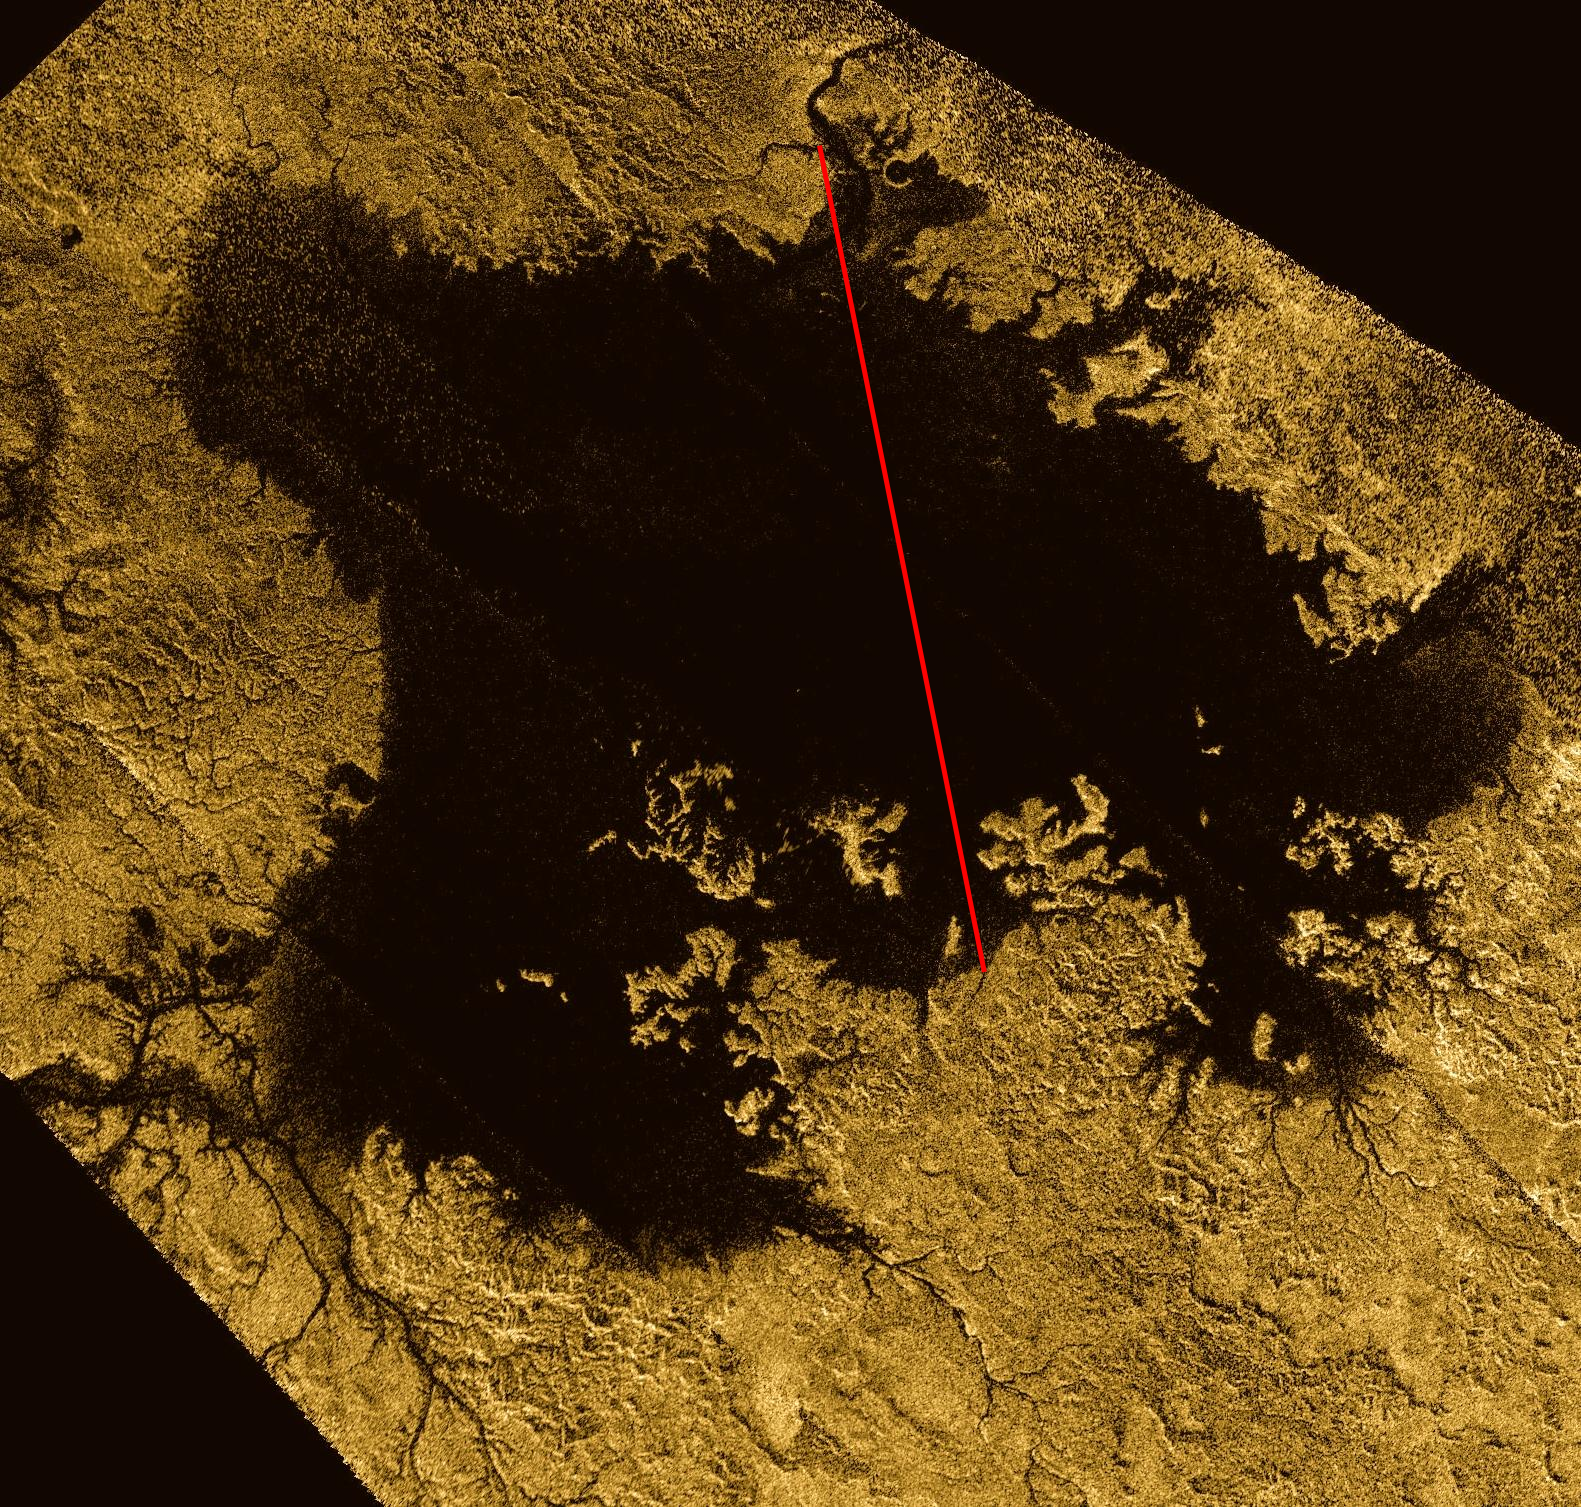
\includegraphics[width=7.8cm]{images/LigeiaMare}
\end{center}
{\tiny \it Radar Image Credit: NASA/JPL-Caltech\\http://www.ciclops.org//view\_media.php?id=39071\&js=1}
\end{frame}
\subsection{Lake bathymetry}
%%%%%%%%%%%%%%%%%%%%%%%%%%%%%%%%%%%%%%%%%%%%%%%%%%%%%%%%%%%%%%%%%%%%
\begin{frame}[fragile]{Lake bathymetry radar altimetry}

\begin{center}
  \includegraphics[width=8.5cm]{images/Mastrogiuseppe2}
\end{center}
\noindent {\tiny \it Figure Credit: Mastrogiuseppe et al. (2014)}
\end{frame}

%%%%%%%%%%%%%%%%%%%%%%%%%%%%%%%%%%%%%%%%%%%%%%%%%%%%%%%%%%%%%%%%%%%%
\begin{frame}[fragile]{Lake bathymetry depth}

\begin{center}
  \includegraphics[width=10cm]{images/MastrogiuseppeLigeiaMare}
\end{center}
\noindent {\tiny \it Figure Credit: Mastrogiuseppe et al. (2014)}
\end{frame}
\subsection{Evaporation}
%%%%%%%%%%%%%%%%%%%%%%%%%%%%%%%%%%%%%%%%%%%%%%%%%%%%%%%%%%%%%%%%%%%%
\begin{frame}[fragile]{Evaporation}
\begin{block}{Evaporation}
20mm/week at poles\\
1mm/week at equator\\
\end{block}
\begin{block}{The vaporization heat adapted to Titan:}
\begin{equation}
H_L = \frac {n_a L}{\eta} C \left( q_s - q_a \right) =  \frac {n_a L}{\eta} C \delta q
\end{equation}
$\eta$ the Avogadro's number\\
L the latent heat of vaporization of methane\\
C the bulk transfer coefficient\\
q the mole fraction of methane at liquid surface (saturated state: $q_s$) and at a given height (typically few meters) in the atmosphere above ($q_a$)
\end{block}
\end{frame}

\section{Rainfall/Run-off}
\subsection{Rainfall}
%%%%%%%%%%%%%%%%%%%%%%%%%%%%%%%%%%%%%%%%%%%%%%%%%%%%%%%%%%%%%%%%%%%%
\begin{frame}[fragile]{Rainfall on Belet (-5N,255E)}
\begin{block}{Rainfall on Belet (-5N,255E)}
The change of surface albedo from Cassini VIMS, darkening after a large cloud passed on the Belet Albedo feature, and brightening again after some time.
\begin{center}
  \includegraphics[width=10cm]{images/WetBeletStormInBeletWithoutOutline150111}
  \vspace{5mm}
  \includegraphics[width=10cm]{images/WetBeletStormInBeletAnnotatedHighRes150111}
\end{center}
{\tiny \it Radar Image Credit: NASA/JPL-Caltech/SSI\\http://www.titanexploration.com/TitanImages2011Plus/TitanImages2011.htm}
\end{block}
\end{frame}

\subsection{ITCZ}
%%%%%%%%%%%%%%%%%%%%%%%%%%%%%%%%%%%%%%%%%%%%%%%%%%%%%%%%%%%%%%%%%%%%
\begin{frame}[fragile]{ITCZ}

\begin{center}
  \includegraphics[width=10cm]{images/TokanoPerspectiveFigure}
\end{center}
\noindent {\tiny \it Figure Credit: Tokano (2013)}
\end{frame}
\section{Conclusions}
%%%%%%%%%%%%%%%%%%%%%%%%%%%%%%%%%%%%%%%%%%%%%%%%%%%%%%%%%%%%%%%%%%%%
\begin{frame}[fragile]{Conclusions}
The (m)ethonological cycle, its energy budget and spatio-temporal dynamics are just starting to be discovered.
\begin{block}{Now}
Every additional fly-by of Cassini\\
Treasure trove for Titan science
\end{block}
\begin{block}{Future missions}
\begin{itemize}
 \item {\bf Rainfall:} microwave sensor on-board orbiter/lander \\~~~~~~~~~~(TRMM type)
 \item {\bf Run-off:} orbital radar altimeter \\~~~~~~~~~~(Magellan Venus radar type)
 \item {\bf Geomorphology:} sub-clouds aerial Lidar altimeter + multi/hyperspectral (TSSM/Mongolfi\`ere type)
 \item {\bf Energy budget:} Thermal profiler in orbit, vessel on lakes/oceans (TSSM/TiME type)
\end{itemize}
\end{block}
\end{frame}

%%%%%%%%%%%%%%%%%%%%%%%%%%%%%%%%%%%%%%%%%%%%%%%%%%%%%%%%%%%%%%%%%%%%
\begin{frame}[fragile]{Thank You}
\begin{block}{Thank you}
\begin{center}
  \includegraphics[width=8.5cm]{images/T91_nice}
\end{center}
{\tiny \it Radar Image Credit: PDS/NASA/JPL-Caltech}
\end{block}
\end{frame}

\end{document}
